\newpage
\section{Problemas}

\question{
  A Figura~\ref{fig:q7} apresenta o losango EFGH inscrito no retângulo ABCD,
  sendo O o ponto de interseção das diagonais desse losango. Decidir se é
  verdadeira ou falsa cada uma das seguintes afirmações:

  \begin{figure}[H]
    \centering
    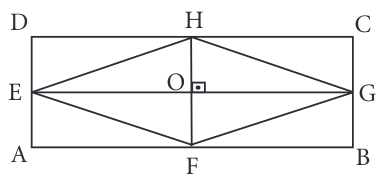
\includegraphics[width=0.5\textwidth]{./fig/q7.png}
    \caption{}\label{fig:q7}
  \end{figure}
}
\begin{center}
  % First column
  \begin{minipage}[t]{0.24\textwidth}
    \begin{itemize}
      \item \subquestion{$\overrightarrow{\mathrm{EO}} = \overrightarrow{\mathrm{OG}}$} \answer{V}
      \item \subquestion{$\overrightarrow{\mathrm{AF}} = \overrightarrow{\mathrm{CH}}$} \answer{F}
      \item \subquestion{$\overrightarrow{\mathrm{DO}} = \overrightarrow{\mathrm{HG}}$} \answer{V}
      \item \subquestion{\vfill$|\mathrm{C - O}| = |\mathrm{O - B}|$} \answer{V}
      \item \subquestion{\vfill$|\mathrm{H - O}| = |\mathrm{H - D}|$} \answer{F}
    \end{itemize}
  \end{minipage}
  \hfill
  % Second column
  \begin{minipage}[t]{0.24\textwidth}
    \begin{itemize}
      \item \subquestion{\vfill$\mathrm{H - E} = \mathrm{O - C}$} \answer{F}
      \item \subquestion{$|\overrightarrow{\mathrm{AC}}| = |\overrightarrow{\mathrm{BD}}|$} \answer{V}
      \item \subquestion{$|\overrightarrow{\mathrm{OA}}| = \frac{1}{2}|\overrightarrow{\mathrm{DB}}|$} \answer{V}
      \item \subquestion{$\overrightarrow{\mathrm{AF}} \parallel \overrightarrow{\mathrm{CD}}$} \answer{V}
      \item \subquestion{$\overrightarrow{\mathrm{GF}} \parallel \overrightarrow{\mathrm{HG}}$} \answer{F}
    \end{itemize}
  \end{minipage}
  \hfill
  % Third column
  \begin{minipage}[t]{0.24\textwidth}
    \begin{itemize}
      \item \subquestion{$\overrightarrow{\mathrm{AO}} \parallel \overrightarrow{\mathrm{OC}}$} \answer{V}
      \item \subquestion{$\overrightarrow{\mathrm{AB}} \perp \overrightarrow{\mathrm{OH}}$} \answer{V}
      \item \subquestion{$\overrightarrow{\mathrm{EO}} \perp \overrightarrow{\mathrm{CB}}$} \answer{V}
      \item \subquestion{$\overrightarrow{\mathrm{AO}} \perp \overrightarrow{\mathrm{HF}}$} \answer{F}
      \item \subquestion{$\overrightarrow{\mathrm{OB}} = -\overrightarrow{\mathrm{FE}}$} \answer{V}
    \end{itemize}
  \end{minipage}
\end{center}

\newpage
\question{Decidir se é verdadeira ou falsa cada uma das afirmações:}
\begin{center}
  % First column
  \begin{minipage}[t]{0.48\textwidth}
    \begin{itemize}
      \item \subquestion{Se $\vec{u} = \vec{v}$, então $|\vec{u}| = |\vec{v}|$.} \answer{V}
      \item \subquestion{Se $|\vec{u}| = |\vec{v}|$, então $\vec{u} = \vec{v}$.} \answer{F}
      \item \subquestion{Se $\vec{u} \parallel \vec{v}$, então $\vec{u} = \vec{v}$.} \answer{F}
      \item \subquestion{Se $\vec{u} = \vec{v}$, então $\vec{u} \parallel \vec{v}$.} \answer{V}
      \item \subquestion{Se $\vec{w} = \vec{u} + \vec{v}$, então $|\vec{w}| = |\vec{u}| + |\vec{v}|$.} \answer{F}
      \item \subquestion{$|\vec{w}| = |\vec{u}| + |\vec{v}|$, então $\vec{u}$, $\vec{v}$ e $\vec{w}$ são paralelos.} \answer{V}
    \end{itemize}
  \end{minipage}
  \hfill
  % Second column
  \begin{minipage}[t]{0.48\textwidth}
    \begin{itemize}
      \item \subquestion{Se $\overrightarrow{\mathrm{AB}} = \overrightarrow{\mathrm{DC}}$, então ABCD (nessa ordem) é paralelogramo.} \answer{V}
      \item \subquestion{$|5\vec{v}| = |-5\vec{v}| = 5|\vec{v}|$.} \answer{V}
      \item \subquestion{Os vetores $3\vec{v}$ e $-4\vec{v}$ são paralelos e de mesmo sentido.} \answer{F}
      \item \subquestion{Se $\vec{u} \parallel \vec{v}$, $|\vec{u}| = 2$ e $|\vec{v}| = 4$, então $\vec{v} = 2\vec{u}$ ou $\vec{v} = -2\vec{u}$.} \answer{V}
      \item \subquestion{Se $|\vec{v}| = 3$, o versor de $-10\vec{v}$ é $-\frac{\vec{v}}{3}$.} \answer{V}
    \end{itemize}
  \end{minipage}
\end{center}

\newpage
\question{Com base na Figura~\ref{fig:q7}, determinar os vetores a seguir, expressando-os com 
origem no ponto A:}
\begin{center}
  % First column
  \begin{minipage}[t]{0.32\textwidth}
    \begin{itemize}
      \item \subquestion{$\overrightarrow{\mathrm{OC}} +
        \overrightarrow{\mathrm{CH}}$} \answer{\overrightarrow{\mathrm{AE}}}
      \item \subquestion{$\overrightarrow{\mathrm{EH}} +
        \overrightarrow{\mathrm{FG}}$} \answer{\overrightarrow{\mathrm{AC}}}
      \item \subquestion{$2\overrightarrow{\mathrm{AE}} +
        2\overrightarrow{\mathrm{AF}}$} \answer{2\overrightarrow{\mathrm{AO}}}
      \item \subquestion{$\overrightarrow{\mathrm{EH}} +
        \overrightarrow{\mathrm{EF}}$} \answer{\overrightarrow{\mathrm{AB}}}
    \end{itemize}
  \end{minipage}
  \hfill
  % Second column
  \begin{minipage}[t]{0.32\textwidth}
    \begin{itemize}
      \item \subquestion{$\overrightarrow{\mathrm{EO}} +
        \overrightarrow{\mathrm{BG}}$} \answer{\overrightarrow{\mathrm{AO}}}
      \item \subquestion{$2\overrightarrow{\mathrm{OE}} +
        2\overrightarrow{\mathrm{OC}}$} \answer{2\overrightarrow{\mathrm{AE}}}
      \item \subquestion{$\frac{1}{2}\overrightarrow{\mathrm{BC}} +
        \overrightarrow{\mathrm{BC}}$} \answer{\overrightarrow{\mathrm{AD}} + \overrightarrow{\mathrm{AE}}}
    \end{itemize}
  \end{minipage}
  \hfill
  % Third column
  \begin{minipage}[t]{0.32\textwidth}
    \begin{itemize}
      \item \subquestion{$\overrightarrow{\mathrm{FE}} +
        \overrightarrow{\mathrm{FG}}$} \answer{\overrightarrow{\mathrm{AD}}}
      \item \subquestion{$\overrightarrow{\mathrm{OG}} -
        \overrightarrow{\mathrm{HO}}$} \answer{\overrightarrow{\mathrm{AO}}}
      \item \subquestion{$\overrightarrow{\mathrm{AF}} +
        \overrightarrow{\mathrm{FO}} + \overrightarrow{\mathrm{AO}}$}
        \answer{\overrightarrow{\mathrm{AC}}}
    \end{itemize}
  \end{minipage}
\end{center}

\question{
  O paralelogramo $ABCD$ (Figura~\ref{fig:q10}) é determinado pelos vetores
  $\overrightarrow{\mathrm{AB}}$ e $\overrightarrow{\mathrm{AD}}$, sendo $M$ e
  $N$ os pontos médios dos lados $\overline{DC}$ e $\overline{AB}$,
  respectivamente. Determinar:

  \begin{figure}[H]
    \centering
    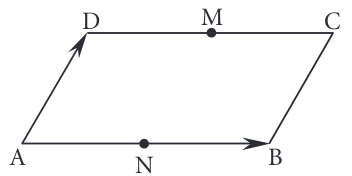
\includegraphics[width=0.5\textwidth]{./fig/q10.png}
    \caption{}\label{fig:q10}
  \end{figure}
}
\begin{center}
  % First column
  \begin{minipage}[t]{0.32\textwidth}
    \begin{itemize}
      \item \subquestion{$\overrightarrow{\mathrm{AD}} +
        \overrightarrow{\mathrm{AB}}$} \answer{\overrightarrow{\mathrm{AC}}}
      \item \subquestion{$\overrightarrow{\mathrm{BA}} +
        \overrightarrow{\mathrm{DA}}$} \answer{\overrightarrow{\mathrm{CA}}}
      \item \subquestion{$\overrightarrow{\mathrm{AC}} -
        \overrightarrow{\mathrm{BC}}$} \answer{\overrightarrow{\mathrm{AB}}}
    \end{itemize}
  \end{minipage}
  \hfill
  % Second column
  \begin{minipage}[t]{0.32\textwidth}
    \begin{itemize}
      \item \subquestion{$\overrightarrow{\mathrm{AN}} +
        \overrightarrow{\mathrm{BC}}$} \answer{\overrightarrow{\mathrm{AM}}}
      \item \subquestion{$\overrightarrow{\mathrm{MD}} +
        \overrightarrow{\mathrm{MB}}$} \answer{\overrightarrow{\mathrm{DN}}}
      \item \subquestion{$\overrightarrow{\mathrm{BM}} -
        \frac{1}{2}\overrightarrow{\mathrm{DC}}$} \answer{\overrightarrow{\mathrm{DB}}}
    \end{itemize}
  \end{minipage}
\end{center}

\question{Apresentar, graficamente, um representante do vetor $\vec{u} -
\vec{v}$ nos casos:

  \begin{figure}[H]
    \centering
    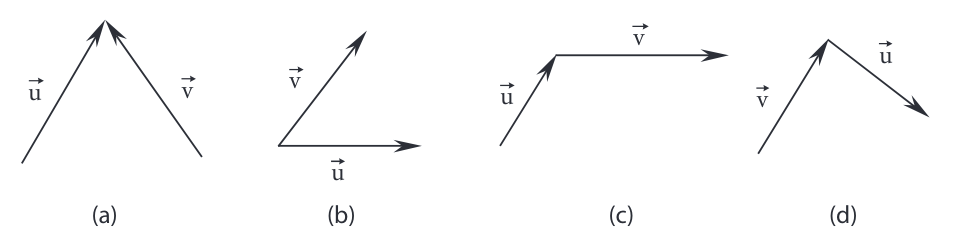
\includegraphics[width=0.6\textwidth]{./fig/fig27.png}
    \caption{}
  \end{figure}
}
\answer{
  \begin{figure}[H]
    \centering
    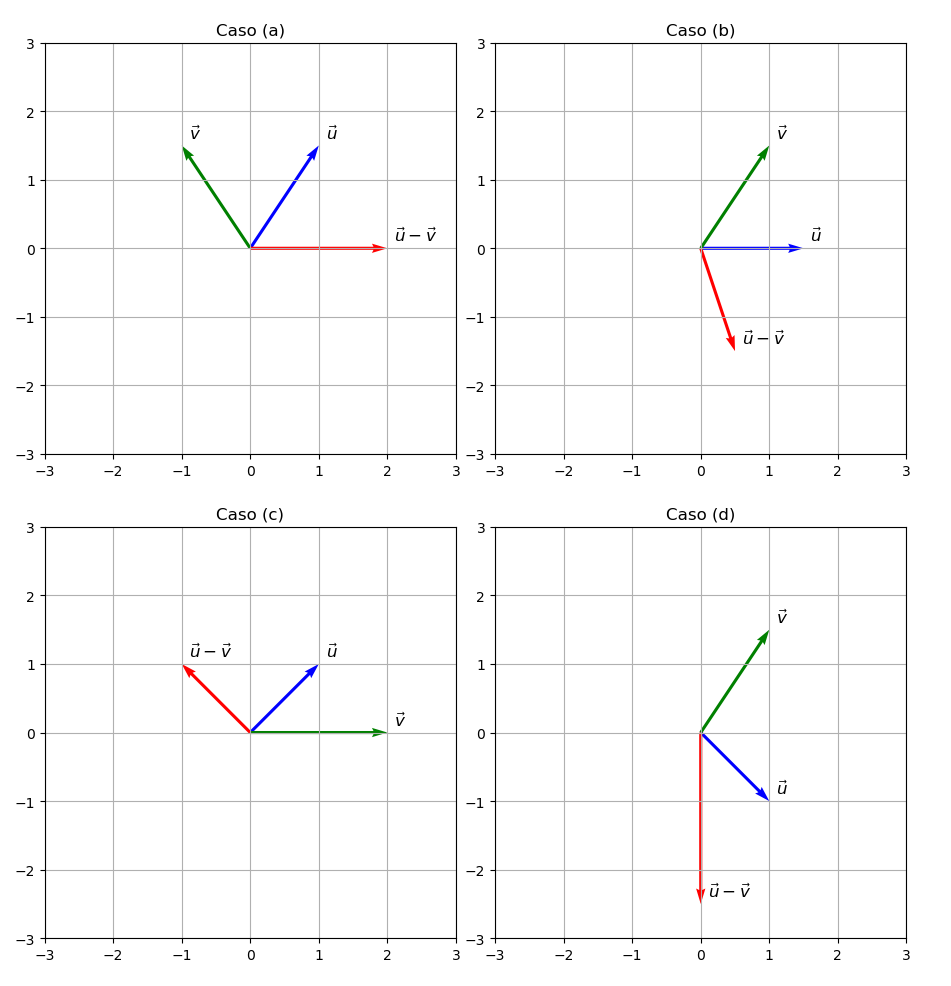
\includegraphics[width=0.75\textwidth]{./fig/q11.png}
    \caption{}
  \end{figure}
}

\newpage
\question{Determinar o vetor $\vec{x}$ nas figuras:

  \begin{figure}[H]
    \centering
    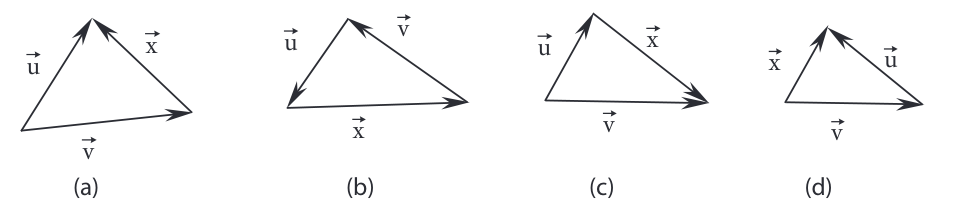
\includegraphics[width=0.6\textwidth]{./fig/q12.png}
    \caption{}
  \end{figure}
}
\subquestion{
  \answer{$\vec{u} - \vec{v}$}
}
\subquestion{
  \answer{$-(\vec{u} + \vec{v})$}
}
\subquestion{
  \answer{$\vec{v} - \vec{u}$}
}
\subquestion{
  \answer{$\vec{u} + \vec{v}$}
}
